\documentclass{article}
\usepackage{fancyhdr}
\usepackage[german]{babel}
\usepackage{mwe}
\usepackage{graphicx}
\pagestyle{fancy}

\author{Philipp Kiss}

\lhead{Philipp Kiss}
\rhead{Information und Codierung}

\begin{document}
\tableofcontents
\newpage

\section{Logikgatter}
\begin{figure}[h]
		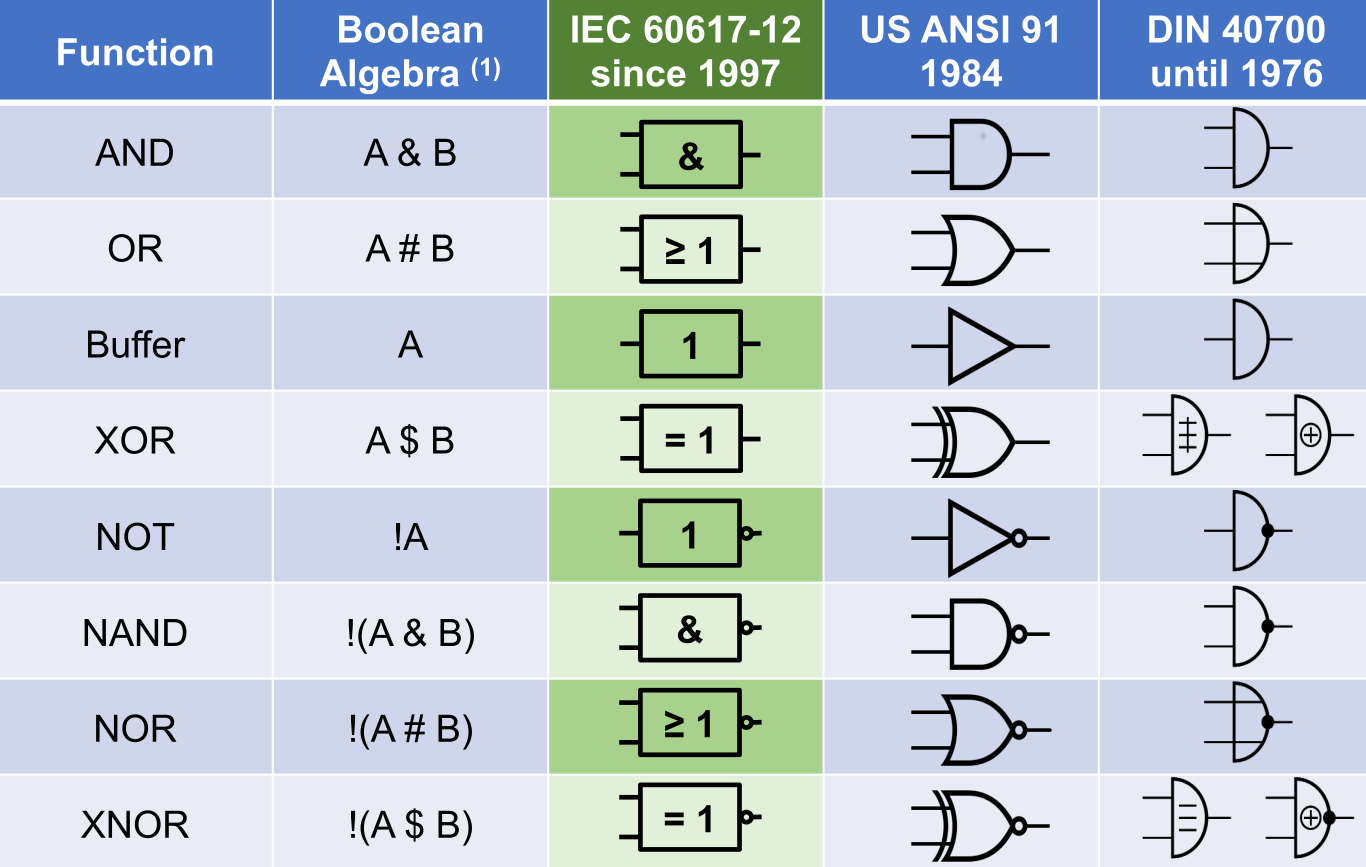
\includegraphics[width=\linewidth]{img/logikgatter.png}
		\caption{verschiedene Logikgatternotationen}
		\label{fig:verschiedene Logikgatternotationen}
\end{figure}
\section{Informationstheorie}
Eine Information ist etwas, was vor seinem Eintreffen noch nicht bekannt war und kann viele Formen annehmen (Ton, Symbol, Text, Wert, ...). Information kann anhand der von ihr beseitigten Unsicherheit gemessen werden. Technisch gesehen ist die kleinste Masseinheit einer Information 1 Bit, sprich eine binäre Entscheidung.
\subsection{Datenquellen}
Eine Datenquelle wird als ``diskret" bezeichnet, wenn sie abzählbare Messwerte liefert. Beispiele dafür sind digitale Sensoren, Ziehung der Lottozahlen, Wetterbericht im Radio. Datenqulle die ``stetig" sind liefern nicht abzählbare Messewerte. Beispiele dafür sind jegliche analoge Messewerte (regeln eines Potentiometers, ablesen eines analogen Thermoeters).

Zudem kann eine Datenquelle ``memoryless" sein, wenn die Messwerte statistisch unabhängig voneinander sind.
\subsection{Formeln}
\paragraph{Die Warscheinlichkeit} einer Information wird errechnet indem man die Vorkommnis der Information durch die gesamten Vorkommnisse teilt. \[
		P(x) = \frac{k(x)}{K} 
\]
\paragraph{Der Informationsgehalt} einer Information wird in Bit angegeben und wird mit \[
		I(x)= \log_{2} \frac{1}{P(x)}
\]
berechnet
\paragraph{Die Entropie} einer Datenquelle bezeichnet den durchschnittlichen Informationsgehalt aller Informationen die diese liefert. Die Masseinheit der Entropie ist Bit/Symbol.
\[
		H(x) = \sum_{n=0}^{N-1} P(x_n) \log_{2} \frac{1}{P(x_n)}
\]
\paragraph{Die Mittlere Codelänge} einer Datenquelle beschreibt die durchschnittliche Bitanzahl, die benötigt wird ein Zeichen der Quelle anzuzeigen.
\[
		L = \sum_{n=0}^{N-1} P(x_n) \cdot l_n 
\]
\paragraph{Die Redundanz} einer Datenquelle bestimmt die Ineffizienz der Bitnutzung. \[
		R = L(x) - H(x)
\]

\section{Quellencodierung}
Das Ziel der Kompression ist, redundante und je nach Standard auch irrelevante Informationen zu minimieren um Ressourcen (Zeit, Energie, Bandbreite) zu sparen.
\subsection{Huffman tree}
Der Huffmantree bietet eine garantiert optimale Codierung. Das heisst eine Codierung mit der geringstmöglichen Redundanz. Dafür ordnet man alle Zeichen nach absteigender Probabilität und verbindet die kleinste Probabilität und die nächstgrössere zu einem Ast. Auf diesem addiert man die beiden Probabilitäten und ordnet den Ast neu ein. Diesen Vorgang wiederholt man, bis man an der Wurzel angekommen ist. Zur Überprüfung: die Summe aller Probabilitäten in der Wurzel muss 1 ergeben.
\section{Mediakompression}
\subsection{JPEG}
Das JPEG-Kompressionsverfahren ist ein \textbf{verlustbehafteter} Kompressionsalgorithmus, welcher sich zur komprimierung natürlicher Bilder eignet. Der JPEG-Algorithmus umfasst 7 Schritte.
\subsubsection{Farbraumtransformation}
Unser Auge ist empflindlicher auf Helligkeitsunterschiede als auf Farbunterschiede. Das ermöglicht eine stärkere verlustbehaftete Kompression der Farben bevor wir markante Unterschiede feststellen können. Deshalb trennen wir die 3 Farbelemente aus dem RGB Farbraum auf in eine Helligkeitskomponente, einen Grün-Rot-Wert und einen Grün-Blau-Wert. Das das grüne Farbspektrum bleibt so stäker erhalten, da wir evolutionär bedingt empfindlicher auf Grünabstufungen sind als für andere Farben. Deshalb trennen wir die 3 Farbelemente aus dem RGB Farbraum auf in eine Helligkeitskomponente, einen Grün-Rot-Wert und einen Grün-Blau-Wert. Das das grüne Farbspektrum bleibt so stäker erhalten, da wir evolutionär bedingt empfindlicher auf Grünabstufungen sind als für andere Farben.
Die Y-Komponente entspricht dem Graustufenbild des Ursprungbildes.
\begin{figure}[h!]
		\begin{center}
		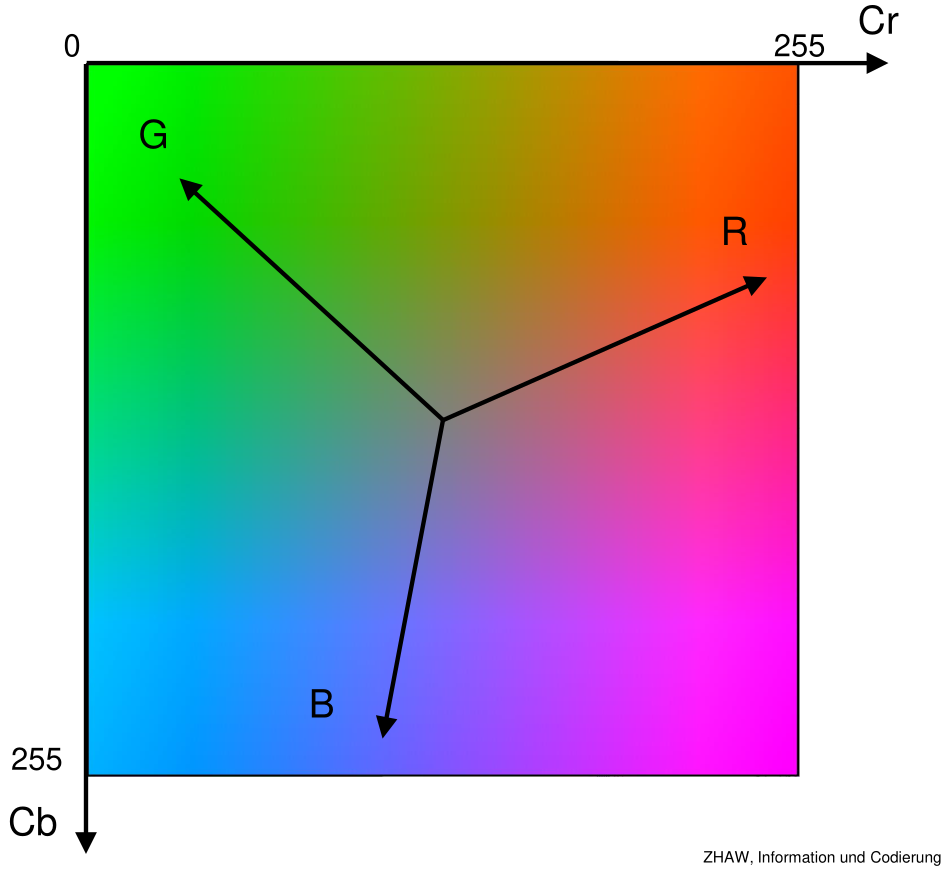
\includegraphics[width=7cm]{img/cbcr.png}
		\end{center}
		\caption{Verhältnis Cb zu Cr}
		\label{fig:Verhältnis Cb zu Cr}
\end{figure}
\subsubsection{Chrominanz Downsampling}
Unter dem Chrominanz Downsampling versteht man das Zusammenfassen mehrere Pixel der Farbebenen. Hier werden das erste Mal irrelevante Informationen ``eliminiert''. 
\begin{figure}[h]
		\begin{center}
		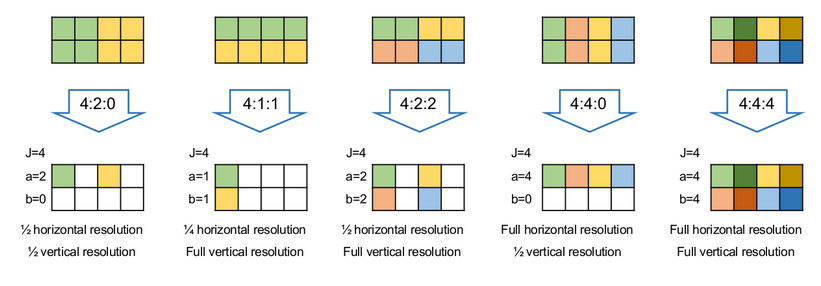
\includegraphics[width=\linewidth]{img/downsampling.png}
		\end{center}
		\caption{Chrominanz Downsampling}
		\label{fig:Chrominanz Downsampling}
\end{figure}
\subsubsection{Pixel-Gruppierung}
Die Idee der nächsten Schritte ist, kleine Pixelgruppierungen möglichst effizient abzuspeichern. Dafür wird das jeder Informationskanal in 8x8 Pixelblöcke aufgeteilt, die dann jeweils gemeinsam komprimiert werden. Falls ein Kanal nicht sauber in 8x8 Pixelblöcke unterteilt werden kann, wird bei den inkompleten Blöcken am Rand entweder die letzte Spalte oder Zeile dupliziert, bis der Block voll ist oder den fehlenden Blöcken wird ein fixer Wert 0 zugewiesen. Beide Optionen führen zu kleinen, kaum spürbaren Artefakten an den Rändern.
\newpage
\subsubsection{Diskrete Cosinustransformation}
Dieser Schritt dient zur Übersetzung der Informationskanäle von Werten von 0-255 zu einer Kombination aus Cosinusfunktionen mit variiernder Frequenz und ist komplett verlustfrei. 
Die Pixelblöcke werden einer nach dem anderen zu einer gewichteten Addition der Cosinusfunktionen übersetzt, da die Koeffizienten weniger Speicherplatz benötigen als die Werte der einzelnen Pixel selbst.

\begin{figure}[h]
    \centering
    \begin{minipage}{0.45\textwidth}
        \centering
        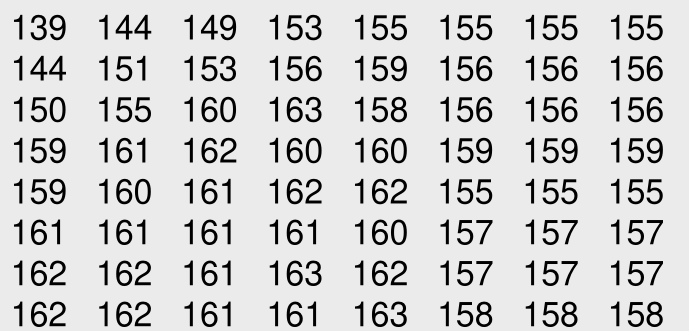
\includegraphics[width=0.9\textwidth]{img/8x8_array.png} 
        \caption{8x8 Pixelarray}
    \end{minipage}\hfill
    \begin{minipage}{0.45\textwidth}
        \centering
        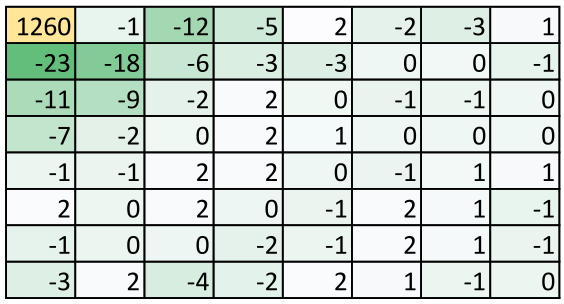
\includegraphics[width=0.9\textwidth]{img/dct_result.png} 
        \caption{8x8 Frequenzarray}
    \end{minipage}
\end{figure}

Es findet also bereits eine verlustfreie Kompression statt. Für die Kompression verwendet man die Forward DCT über dem 2 dimensionalen 8x8-Pixelblock Array und erhält daraus für jeden Pixelblock ein 2 dimensionales Frequenzarray indem die jeweiligen Koeffizienten festgehalten werden. Die Forward DCT sieht wie folgt aus:
$$F_{vu} = \frac{1}{4} C_u C_v \sum_{x=0}^7 \sum_{y=0}^7 B_{yx} \cos \left( \frac{(2x+1)u\pi}{16} \right) \cos \left( \frac{(2y+1)v\pi}{16} \right)$$
\begin{figure}[h]
		\begin{center}
		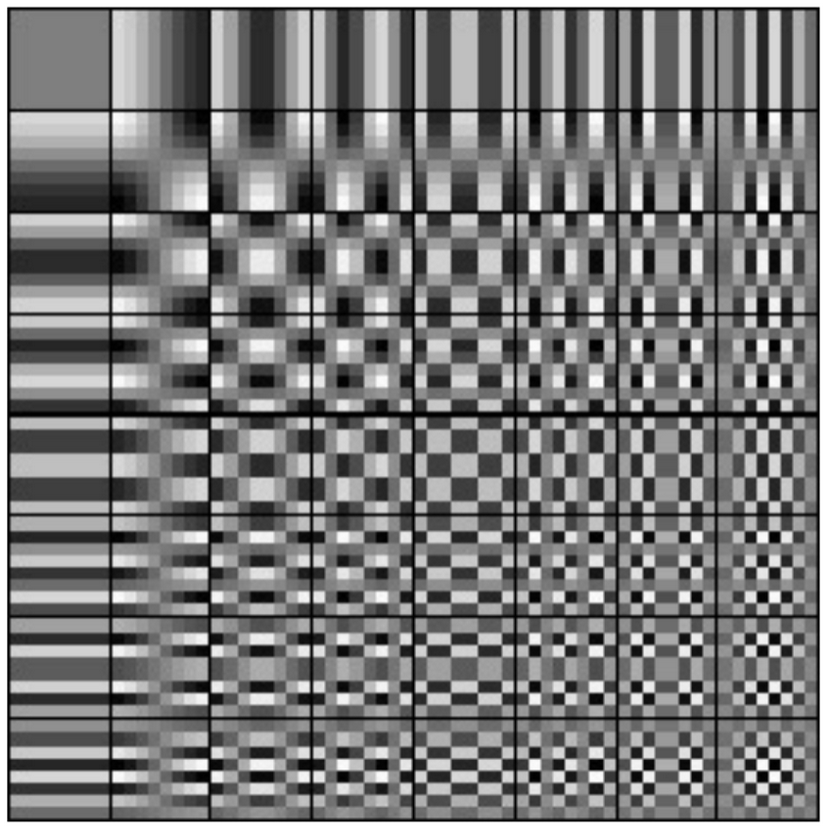
\includegraphics[width=6.5cm]{img/dct.png}
		\end{center}
		\caption{8x8 Cosinusfunktionsmatrix}
		\label{fig:8x8 Cosinusfunktionsmatrix}
\end{figure}
\newpage
\subsubsection{Quantisierung}
Die Quantisierung ist der letzte verlustbehaftete Schritt im ganzen Kompressionsverfahren. Hierfür verwendet man je nach gewünschter Kompression eine tolerantere oder eine aggressivere Quantisierungstabelle. Eine Quantisierungstabelle ist eine Tabelle die analog zu den Pixelblöcken 8x8 Werte beinhaltet, wobei die Werte oben links tiefer sind und gegen unten und gegen rechts höher werden. Indem man alle Werte des Frequenzarrays durch den entsprechenden Quantisierungskoeffizienten teilt und das Resultat auf die nächste ganze Zahl rundet erhält man die Quantisierte Koeffiziententabelle. Dabei gehen feine Unterschiede, die in der ursprünglichen Frequenztabelle unten rechts waren verloren, da sie durch höhere Werte geteilt werden, welche dann auf 0 abgerundet werden. Die massgebenden Frequenzen bleiben dabei besser erhalten.
\begin{figure}[h]
		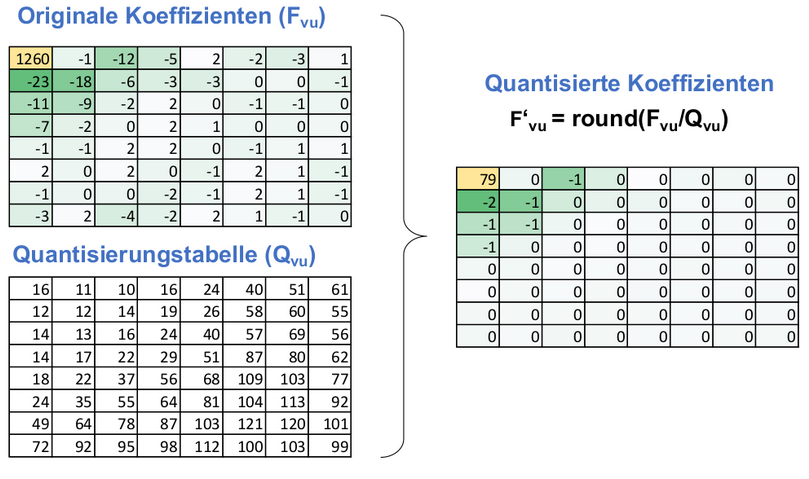
\includegraphics[width=\linewidth]{img/quantisierung.png}
		\caption{Quantisierung}
		\label{fig:Quantisierung}
\end{figure}
\newpage
\subsubsection{Entropy-Coding}
Die Entropiecodierung dient dem effizienten speichern der quantifizierten Koeffizententabelle. Da oben rechts tendenziell höhere Werte sind und unten linke mehr 0 Werte, wird die Matrix in einem Zick-Zack-Muster durchlaufen und diese Tokens mithilfe eines RLE-Verfahrens gespeichert. Das RLE-Verfahren ist im JPEG-Algorithmus nicht genau vorgegeben.
\begin{figure}[h]
		\begin{center}
		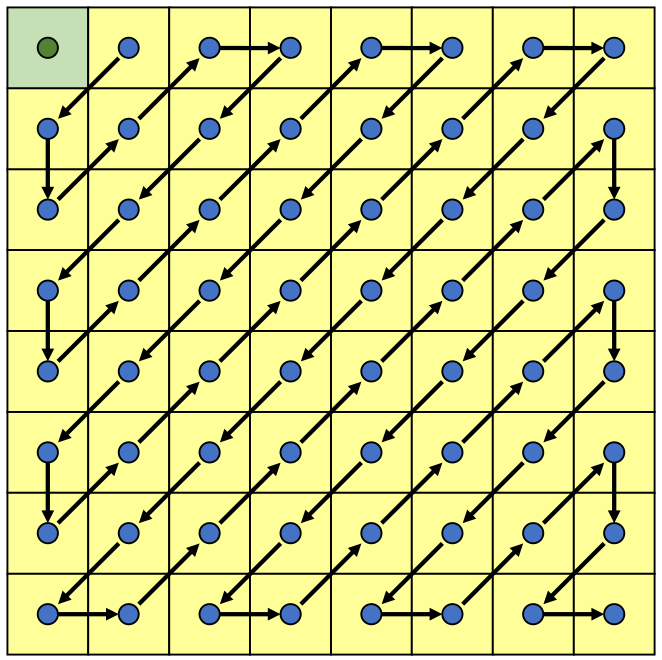
\includegraphics[width=5cm]{img/zigzag.png}
		\end{center}
		\caption{Zick-Zack durchlauf}
		\label{fig:Zick-Zack durchlauf}
\end{figure}
\subsubsection{In Datei verpacken}
Alle Werte die benötigt werden, um das Bild wieder herzustellen werden nun in eine .jpg Datei gespeichert. Das beinhaltet die komprimierte Koeffizentenmatrix sowie die genutzte Quantisierungstabelle und die entsprechenden Anhaltspunkte zum genutzten RLE-Verfahren.

\subsection{Audiokompression}
Schallwellen sind analoge Werte, welche zur Speicherung oder Bearbeitung in digitale Werte umgewandelt werden müssen. Dafür ``tastet'' man die analoge Frequenz ab und arbeitet mit diesen Werten weiter.
\subsubsection{Abtasten}
Das Shannon (oder Shannon-Nyquist Theorem) besagt, dass die Abtastfrequenz für ein Signal mit höchster Frequenzkomponente $\omega$ grösser als $2\omega$ sein muss,um das Signal garantiert verlustfrei abzubilden. Das menschliche Gehör kann Frequenzen bis zu ca. 22kHz verzeichnen, was jedoch von Gehör zu Gehör unterschiedlich ist. Deshalb wird in der Unterhaltung oft mit einer Abtastrate von 44.1kHz oder höher gearbeitet, da wir Frequenzen über 22kHz, die mit einer solchen Abtastrate verloren gehen, sowieso nicht hören würden.

\subsubsection{Quantisierung}
Mit der Quantisierung wird die Amplitude der Abtastpunkte festgehalten. Da das eingehende Signal stetig ist, wir jedoch nur mit diskreten Werten arbeiten können, geht hier unweigerlich Information verloren. Die Auflösung der Quantisierung bestimmt, wie viele höhen-Abstufungen für die Amplitude der Frequenz gespeichert werden. Die Werte, welche nicht genau auf einer Höhenabstufung liegen, werden zur nächsten Abstufung auf- beziehugnsweise abgerundet.
\begin{figure}[h]
		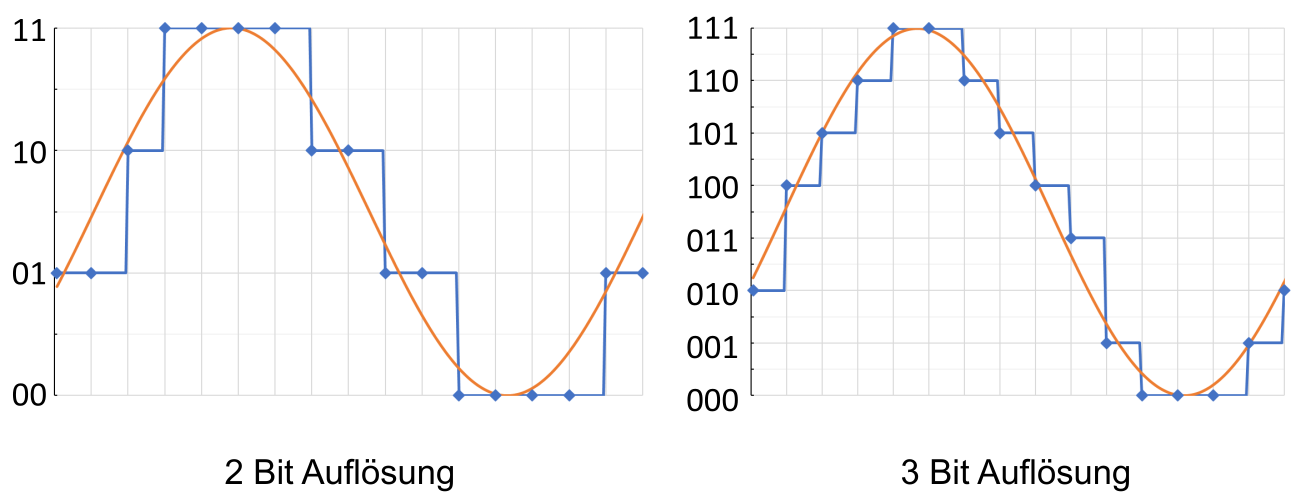
\includegraphics[width=\linewidth]{img/audioQuantisierung.png}
		\caption{Quantisierung eines analogen Signals}
		\label{fig:Quantisierung eines analogen Signals}
\end{figure}
\newline
Bei einer Umwandlung von stetigen zu diskreten Werten entsteht ein Rauschen, so auch bei der Konvertierung von analogen zu digitalen Signalen. Dieses Quantisierungsrauschen ist die Differenz des Rohsignals zu dem digitalen Signal. Daraus folgt, je feiner die diskreten Werte granulier sind, desto kleiner ist auch das Rauschen. Die Lautstärke des Rauschens beträgt $6\textrm{dB} \cdot \textrm{Anzahl Bit}$
\subsubsection{Pulsecode Modulierung}

\end{document}
